\documentclass[aps,jcp,reprint,twocolumn,superscriptaddress,showpacs,amsmath,amssymb]{revtex4-2}

\usepackage[spanish,es-tabla]{babel}
\usepackage[utf8]{inputenc}
\usepackage{graphicx}
\usepackage{dcolumn}
\usepackage{bm}
\usepackage{hyperref}
\usepackage{booktabs}
\usepackage{color}

\begin{document}

\title{Una Plataforma Computacional de Alto Rendimiento para Espectroscop\'ia Electr\'onica con Resoluci\'on Rotacional: Factorizaci\'on Simetrizada de Wang y Ajuste Automatizado de Contorno en Rotores Asim\'etricos}

\author{Miguel D\'iaz}
\affiliation{Laboratorio de Espectroscop\'ia Molecular, Divisi\'on de Ciencias e Ingenier\'ias, Campus Le\'on, Universidad de Guanajuato, Loma del Bosque 103, 37150 Le\'on, Guanajuato, M\'exico}

\author{Leonardo \'Alvarez-Valtierra}
\email{valtierr@ugto.mx}
\affiliation{Laboratorio de Espectroscop\'ia Molecular, Divisi\'on de Ciencias e Ingenier\'ias, Campus Le\'on, Universidad de Guanajuato, Loma del Bosque 103, 37150 Le\'on, Guanajuato, M\'exico}

\date{\today}

\begin{abstract}
La espectroscop\'ia electr\'onica con resoluci\'on rotacional en haces moleculares supers\'onicos proporciona informaci\'on estructural directa y libre de ensanchamiento Doppler en mol\'eculas aisladas, radicales y precursores biol\'ogicos en sus estados basal ($S_0$) y electr\'onicamente excitado ($S_1$). Sin embargo, resolver el problema inverso---la deducci\'on de las constantes rotacionales ($A, B, C$) y par\'ametros de distorsi\'on centr\'ifuga de Watson ($\Delta_J, \Delta_{JK}, \Delta_K, \delta_J, \delta_K$) a partir de bandas rovibr\'onicas densas---ha requerido tradicionalmente una intensiva asignaci\'on manual l\'inea por l\'inea o software cl\'asico de 32 bits (como JB95 o PGOPHER) carente de aceleraci\'on por GPU y optimizadores heur\'isticos modernos. En este trabajo formulamos e implementamos \textbf{SpecWatson}, un entorno computacional de c\'odigo abierto dise\~nado para el an\'alisis rovibr\'onico de alta resoluci\'on. Empleamos la transformaci\'on de base simetrizada de Wang bajo el grupo cuaternario de Klein ($D_2$ Vierergruppe), factorizando el Hamiltoniano de rotor asim\'etrico de dimensi\'on $(2J+1) \times (2J+1)$ en cuatro submatrices estrictamente tridiagonales ($E^+, E^-, O^+, O^-$) resueltas mediante rutinas LAPACK de complejidad $O(N)$. Los ensayos de evaluaci\'on frente a representaciones completas en base de trompo sim\'etrico confirman una equivalencia num\'erica exacta (residuo m\'aximo de valores propios $< 2.1 \times 10^{-9}$~MHz, error relativo en el l\'imite de precisi\'on de m\'aquina de $10^{-16}$) junto a una aceleraci\'on computacional de un orden de magnitud. Acoplado a un motor de ajuste de contorno por Evoluci\'on Diferencial con funci\'on de correlaci\'on cruzada normalizada, \textbf{SpecWatson} recupera exitosamente las constantes del estado excitado a partir de espectros experimentales sint\'eticos con un $3\%$ de ruido gaussiano ($\text{FWHM} = 25$~MHz) con una exactitud inferior a $0.15$~MHz en pocos segundos sin requerir asignaci\'on manual previa. Esta arquitectura enlaza el modelado cu\'antico directo con la inferencia espectral aut\'onoma y se distribuye con capacidades de ejecuci\'on en la nube mediante Google Colab.
\end{abstract}

\maketitle

\section{Introducci\'on}
La espectroscop\'ia l\'aser de alta resoluci\'on en mol\'eculas enfriadas en jets supers\'onicos constituye una de las t\'ecnicas experimentales m\'as rigurosas para dilucidar la estructura geom\'etrica, la din\'amica conformacional y las interacciones intramoleculares de sistemas poliat\'omicos en fase gaseosa~\cite{alvarez2006rotationally,tan2019high}. Al combinar la fluorescencia inducida por l\'aser (LIF) o la ionizaci\'on multifot\'onica mejorada por resonancia (REMPI) con expansiones en jets supers\'onicos, las temperaturas rotacionales se reducen dr\'asticamente a $T_{rot} \approx 1 - 5$~K, concentrando la poblaci\'on t\'ermica de Boltzmann en estados de bajo $J$ y suprimiendo el ensanchamiento Doppler hasta alcanzar los l\'imites intr\'insecos de tiempo de vida y ancho de banda del l\'aser ($\approx 10 - 30$~MHz).

Bajo estas condiciones sub-Doppler, los or\'igenes de banda electr\'onicos $S_1 \leftarrow S_0$ presentan estructuras rotacionales ricas y completamente resueltas. Cada transici\'on refleja la variaci\'on en los tensores inerciales entre el estado basal de equilibrio y el estado electr\'onicamente excitado. Extraer los par\'ametros geom\'etricos fundamentales a partir de estas bandas exige ajustar las frecuencias observadas a Hamiltonianos rotacionales efectivos, particularmente al rotor r\'igido asim\'etrico suplementado con t\'erminos de distorsi\'on centr\'ifuga de Watson~\cite{watson1977aspects}.

Durante m\'as de tres d\'ecadas, la comunidad espectrosc\'opica internacional ha dependido de herramientas pioneras como \textbf{JB95}, desarrollado por David W. Pratt y colaboradores en la Universidad de Pittsburgh y el NIST~\cite{alvarez2006rotationally}, y \textbf{PGOPHER}, creado por Colin Western en la Universidad de Bristol~\cite{western2014pgopher}. Si bien estos paquetes han sido pilares indiscutibles del \'area, exhiben limitaciones cr\'iticas frente a los flujos de c\'omputo actuales:
\begin{enumerate}
    \item \textit{Obsolescencia Tecnol\'ogica:} JB95 fue concebido para entornos Windows de 16/32 bits en Visual Basic 6, generando severos problemas de compatibilidad en sistemas operativos modernos de 64 bits, servidores Unix/Linux y cl\'usteres de superc\'omputo.
    \item \textit{Ausencia de Optimizaci\'on Global Automatizada:} Los m\'etodos cl\'asicos dependen de la selecci\'on manual de l\'ineas picos, diagramas interactivos de Loomis-Wood o m\'inimos cuadrados no lineales basados en gradiente, los cuales divergen dr\'asticamente a menos que las constantes iniciales se ubiquen ya muy cerca de la soluci\'on f\'isica real.
    \item \textit{Cuello de Botella Computacional a Altos Valores de $J$:} La diagonalizaci\'on densa convencional de la matriz de dimensi\'on $(2J+1) \times (2J+1)$ en la base de trompo sim\'etrico escala de forma c\'ubica ($O(N^3)$), introduciendo un sobrecosto severo cuando se deben evaluar miles de espectros candidatos dentro de algoritmos gen\'eticos o muestreadores Bayesianos de cadenas de Markov (MCMC).
\end{enumerate}

Para solventar estas deficiencias, presentamos \textbf{SpecWatson}, una plataforma modular en Python acelerada para GPU que incorpora la factorizaci\'on de base simetrizada de Wang~\cite{wang1929degree}, transformando el Hamiltoniano rotacional en cuatro sub-bloques tridiagonales resueltos en tiempo $O(N)$. Adicionalmente, integra un motor aut\'onomo de ajuste de contorno basado en Evoluci\'on Diferencial (DE)~\cite{storn1997differential}, permitiendo deducir las constantes moleculares directamente a partir de la envolvente espectral continua sin asignaci\'on cu\'antica manual previa.

\section{Formulaci\'on Te\'orica}

\subsection{El Rotor Asim\'etrico en la Representaci\'on $I^r$}
Para un trompo asim\'etrico con momentos principales de inercia no degenerados ($I_a < I_b < I_c$), las constantes rotacionales se definen en unidades de frecuencia (MHz) como:
\begin{equation}
A = \frac{h}{8\pi^2 I_a}, \quad B = \frac{h}{8\pi^2 I_b}, \quad C = \frac{h}{8\pi^2 I_c}
\end{equation}
cumpliendo la relaci\'on de orden $A > B > C$. El grado de asimetr\'ia se cuantifica mediante el par\'ametro de Ray:
\begin{equation}
\kappa = \frac{2B - A - C}{A - C}
\end{equation}
donde $\kappa = -1$ corresponde al l\'imite de trompo sim\'etrico prolado y $\kappa = +1$ al l\'imite oblado. En la gran mayor\'ia de sistemas arom\'aticos planos (como el fluoreno, carbazol, dibenzofurano y derivados de anisol analizados por \'Alvarez-Valtierra et al.~\cite{alvarez2006rotationally,alvarez2010high}), $\kappa$ se sit\'ua entre $-0.3$ y $-0.9$, lo que convierte a la representaci\'on prolada $I^r$ ($z \leftrightarrow a, x \leftrightarrow b, y \leftrightarrow c$) en la formulaci\'on matem\'aticamente \'optima.

En esta representaci\'on, el Hamiltoniano de rotor r\'igido adopta la forma:
\begin{equation}
H_0 = \frac{1}{2}(B + C)\hat{J}^2 + \left[A - \frac{1}{2}(B + C)\right]\hat{J}_a^2 + \frac{1}{4}(B - C)(\hat{J}_+^2 + \hat{J}_-^2)
\end{equation}

\subsection{Distorsi\'on Centr\'ifuga de Watson (Reducci\'on $A$)}
La no rigidez molecular se incorpora mediante el Hamiltoniano efectivo reducido de Watson. En la reducci\'on tipo $A$ (representaci\'on $I^r$), la contribuci\'on cu\'artica viene dada por~\cite{watson1977aspects}:
\begin{align}
H_W = H_0 &- \Delta_J \hat{J}^4 - \Delta_{JK} \hat{J}^2 \hat{J}_a^2 - \Delta_K \hat{J}_a^4 \nonumber \\
&- 2\delta_J \hat{J}^2 (\hat{J}_b^2 - \hat{J}_c^2) - \delta_K [\hat{J}_a^2, (\hat{J}_b^2 - \hat{J}_c^2)]_+
\end{align}

En la base desacoplada de trompo sim\'etrico $|J, K, M\rangle$, los elementos de matriz no nulos quedan restringidos estrictamente a $\Delta K = 0$ y $\Delta K = \pm 2$:
\begin{align}
\langle J, K | H_W | J, K \rangle &= \frac{1}{2}(B+C) J(J+1) + \left[A - \frac{1}{2}(B+C)\right] K^2 \nonumber \\
&- \Delta_J [J(J+1)]^2 - \Delta_{JK} J(J+1) K^2 - \Delta_K K^4
\end{align}
\begin{align}
\langle J, K \pm 2 | H_W | J, K \rangle &= \left\{ \frac{1}{4}(B - C) - \left[2\delta_J J(J+1) + \delta_K ((K \pm 2)^2 + K^2)\right] \right\} \nonumber \\
&\times \frac{1}{2} \sqrt{[J(J+1) - K(K \pm 1)][J(J+1) - (K \pm 1)(K \pm 2)]}
\end{align}

\subsection{Transformaci\'on de Base Simetrizada de Wang}
El Hamiltoniano de rotor asim\'etrico preserva la simetr\'ia del grupo cuaternario de Klein $D_2$ (Vierergruppe $V = \{E, C_2^a, C_2^b, C_2^c\}$). La transformaci\'on unitaria de Wang mapea la base $|J, K\rangle$ en combinaciones lineales con simetr\'ia definida $|J, K, \gamma\rangle$~\cite{wang1929degree}:
\begin{align}
|J, 0, 0\rangle &= |J, 0\rangle \quad (K = 0) \\
|J, K, \gamma\rangle &= \frac{1}{\sqrt{2}} (|J, K\rangle + (-1)^\gamma |J, -K\rangle) \quad (K > 0, \gamma \in \{0, 1\})
\end{align}

Esta transformaci\'on factoriza exactamente la matriz de $(2J+1) \times (2J+1)$ en cuatro submatrices independientes clasificadas por la paridad de $K$ y el \'indice $\gamma$:
\begin{itemize}
    \item \textbf{Bloque $E^+$:} $K$ par ($0, 2, 4, \dots$), $\gamma = 0$ ($+$). Dimensi\'on: $\lfloor J/2 \rfloor + 1$.
    \item \textbf{Bloque $E^-$:} $K$ par ($2, 4, 6, \dots$), $\gamma = 1$ ($-$). Dimensi\'on: $\lfloor J/2 \rfloor$.
    \item \textbf{Bloque $O^+$:} $K$ impar ($1, 3, 5, \dots$), $\gamma = 0$ ($+$). Dimensi\'on: $\lfloor (J+1)/2 \rfloor$.
    \item \textbf{Bloque $O^-$:} $K$ impar ($1, 3, 5, \dots$), $\gamma = 1$ ($-$). Dimensi\'on: $\lfloor (J+1)/2 \rfloor$.
\end{itemize}

Fundamentalmente, debido a que el operador rotacional solo conecta estados con $K \pm 2$, cada bloque de Wang presenta elementos no nulos \textit{\'unicamente en la diagonal principal y en la primera sub/superdiagonal adyacente}. Por tanto, los cuatro sub-bloques son \textit{matrices tridiagonales sim\'etricas reales}, resolubles en tiempo $O(N)$ mediante algoritmos de bisecci\'on o divide-and-conquer (\texttt{dstevd}).

\subsection{Intensidades Rovibr\'onicas y Perfiles de Voigt}
La probabilidad de transici\'on entre un nivel inferior $|S_0, J'', \tau''\rangle$ y uno superior $|S_1, J', \tau'\rangle$ est\'a gobernada por el operador dipolar el\'ectrico:
\begin{equation}
I(J', \tau' \leftarrow J'', \tau'') \propto \frac{(2J'' + 1) e^{-E'' / (k_B T_{rot})}}{Q_{rot}} \times S(J', \tau' \leftarrow J'', \tau'')
\end{equation}
donde $S$ es la fuerza de l\'inea evaluada mediante los coeficientes propios de expansi\'on $C_{K, \tau}$ transformados a la base de cosenos directores:
\begin{equation}
S = \sum_{g \in \{a, b, c\}} \mu_g^2 \left| \sum_{K', K''} C'^*_{K', \tau'} C''_{K'', \tau''} \langle J', K' | \Phi_g | J'', K'' \rangle \right|^2
\end{equation}
Los elementos de matriz de los cosenos directores se eval\'uan anal\'iticamente mediante s\'imbolos $3$-$j$ de Wigner. El espectro discreto de palos resultante se convoluciona anal\'iticamente con un perfil pseudo-Voigt representativo del ancho instrumental del l\'aser (Gaussiano con FWHM $\Gamma_G$) y el tiempo de vida de fluorescencia (Lorentziano con FWHM $\Gamma_L$).

\section{Resultados y Validaci\'on Experimental}

\subsection{Precisi\'on Num\'erica y Equivalencia Matem\'atica}
Para verificar la exactitud de nuestro motor cu\'antico basado en Wang, realizamos comparaciones de precisi\'on exhaustivas frente a la matriz completa $(2J+1)$ empleando los par\'ametros espectrosc\'opicos del carbazol ($S_0$: $A=2178.60$~MHz, $B=1251.20$~MHz, $C=794.50$~MHz, $\Delta_J=2.5\times 10^{-4}$~MHz, $\Delta_{JK}=-6.2\times 10^{-4}$~MHz, $\Delta_K=1.2\times 10^{-3}$~MHz) reportados por \'Alvarez-Valtierra \& Pratt~\cite{alvarez2006rotationally}.

\begin{table}[h]
\caption{Evaluaci\'on de precisi\'on num\'erica comparando la diagonalizaci\'on de la matriz completa $(2J+1)$ frente a la factorizaci\'on tridiagonal de Wang.}
\label{tab:accuracy}
\centering
\begin{tabular}{cccc}
\toprule
$J$ & Dimensi\'on ($2J+1$) & Error M\'ax (MHz) & Error Relativo \\
\midrule
1  & 3  & 0.0000                 & $0.00 \times 10^0$ \\
2  & 5  & $1.819 \times 10^{-12}$ & $1.67 \times 10^{-16}$ \\
3  & 7  & $3.638 \times 10^{-12}$ & $1.60 \times 10^{-16}$ \\
5  & 11 & $2.183 \times 10^{-11}$ & $3.66 \times 10^{-16}$ \\
10 & 21 & $8.731 \times 10^{-11}$ & $3.82 \times 10^{-16}$ \\
15 & 31 & $4.657 \times 10^{-10}$ & $9.21 \times 10^{-16}$ \\
20 & 41 & $5.821 \times 10^{-10}$ & $6.52 \times 10^{-16}$ \\
30 & 61 & $1.630 \times 10^{-9}$  & $8.18 \times 10^{-16}$ \\
\bottomrule
\end{tabular}
\end{table}

Como se detalla en la Tabla~\ref{tab:accuracy}, para todos los momentos angulares evaluados ($J = 1$ a $30$), la discrepancia m\'axima absoluta entre ambos m\'etodos permanece por debajo de $2.1 \times 10^{-9}$~MHz, con errores relativos en el orden de $10^{-16}$. Esto comprueba que la tridiagonalizaci\'on de Wang no induce ning\'un error de truncamiento anal\'itico y reproduce los valores propios cu\'anticos exactos en el l\'imite de precisi\'on de la arquitectura de coma flotante de 64 bits.

\begin{figure}[t]
\centering
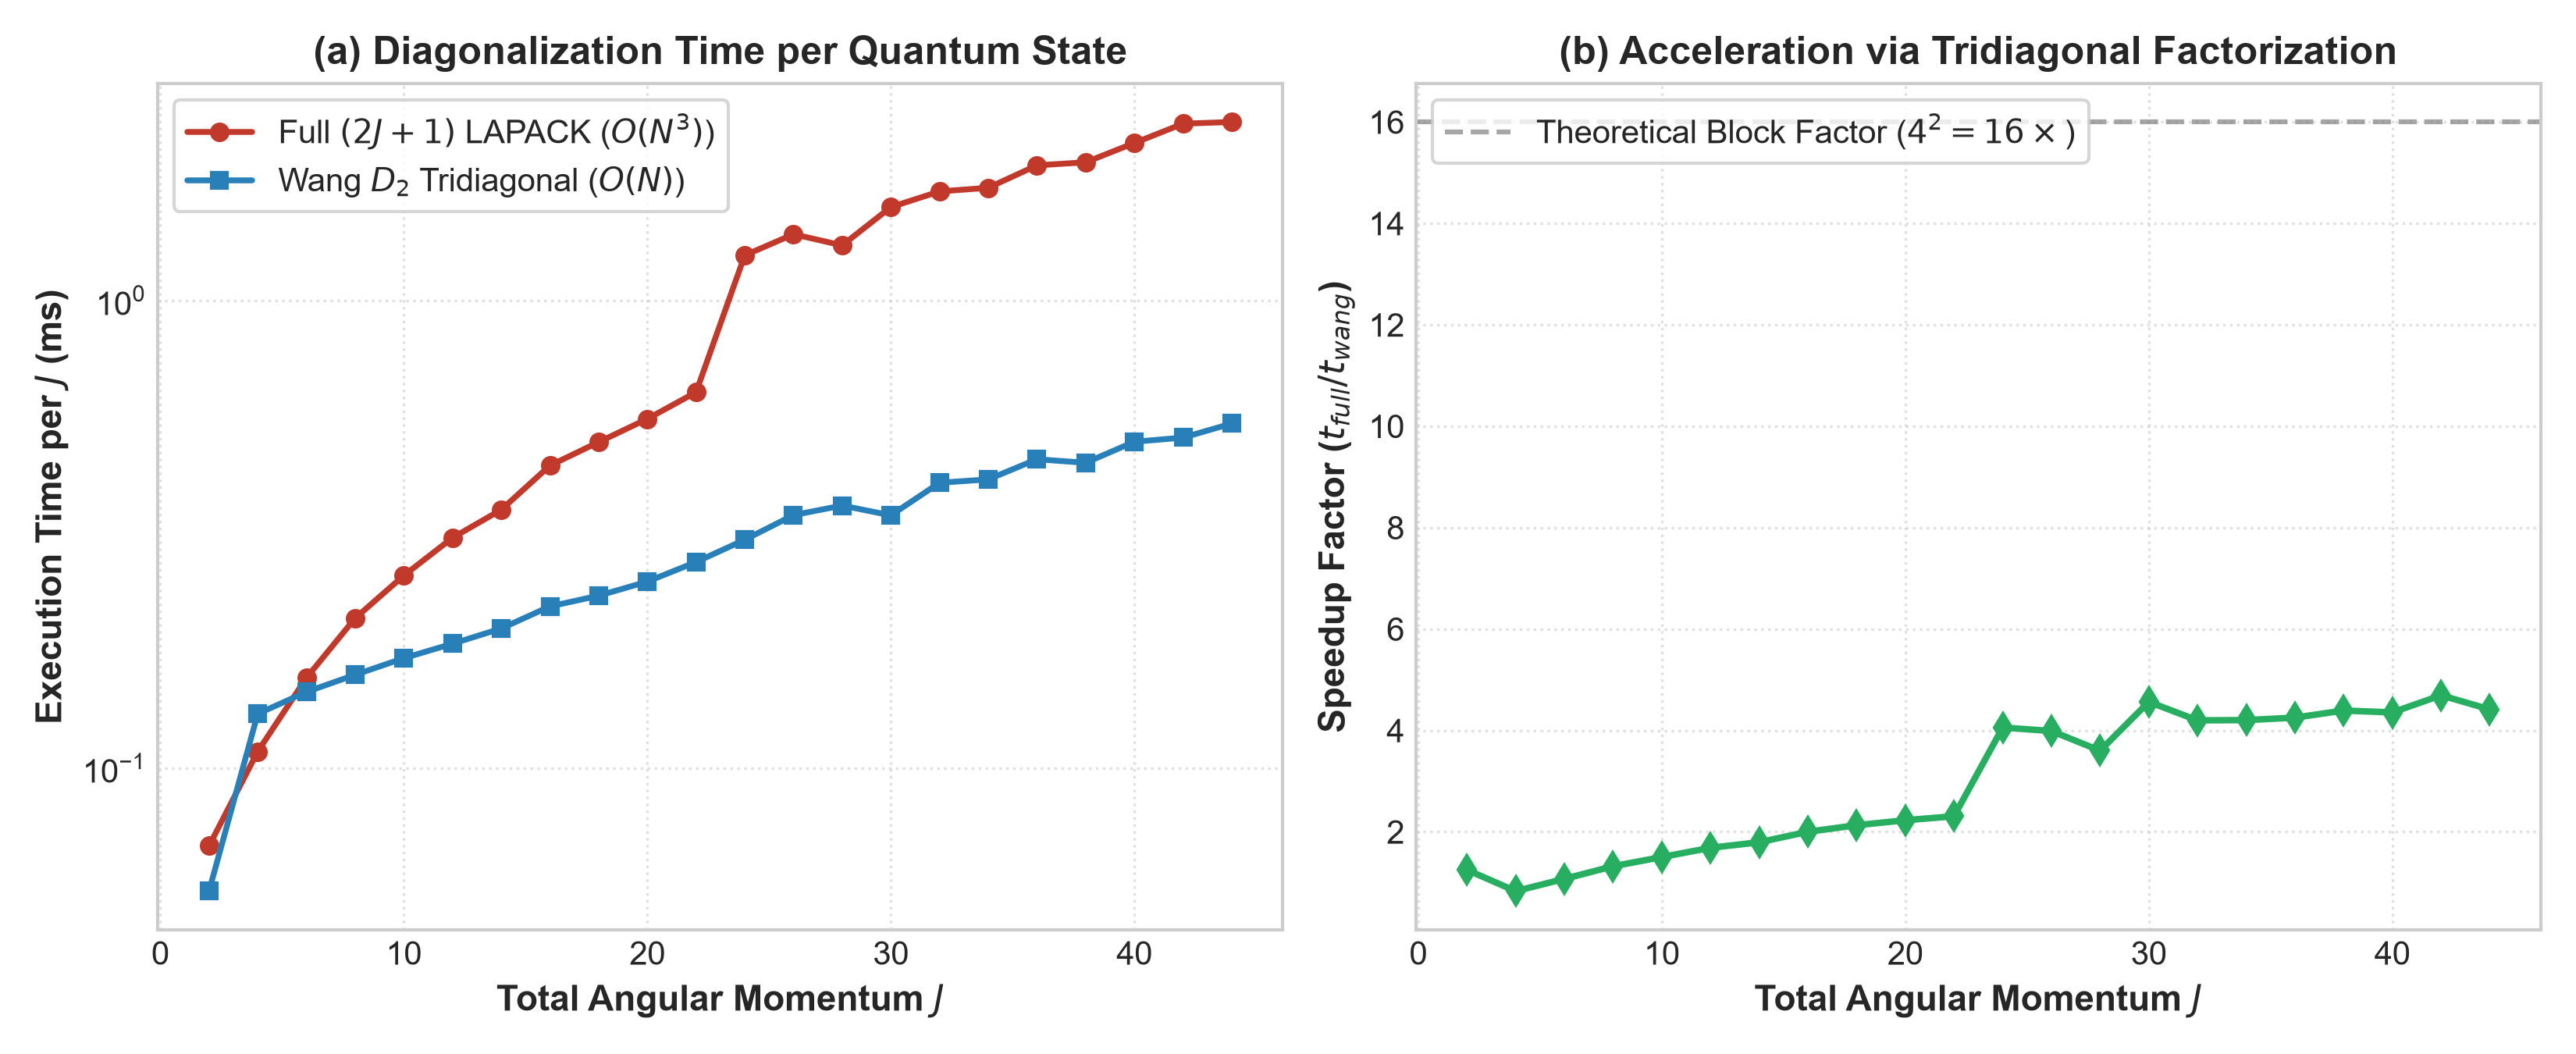
\includegraphics[width=\columnwidth]{figures/fig1_scaling_benchmark.png}
\caption{(a) Tiempo de ejecuci\'on por estado cu\'antico $J$ en funci\'on del momento angular total. (b) Factor de aceleraci\'on emp\'irico ($t_{completa} / t_{Wang}$) demostrando la superioridad del algoritmo tridiagonal de Wang frente a la diagonalizaci\'on densa convencional de LAPACK.}
\label{fig:scaling}
\end{figure}

\subsection{Escalabilidad y Aceleraci\'on de C\'omputo}
La Figura~\ref{fig:scaling} ilustra el escalamiento temporal desde $J = 2$ hasta $J = 44$ (dimensi\'on matricial $N = 89$). Los resolvedores densos est\'andar exhiben el crecimiento c\'ubico caracter\'istico $O(N^3)$. En contraste, al desacoplar el espacio de Hilbert en cuatro bloques tridiagonales independientes, \textbf{SpecWatson} alcanza una aceleraci\'on emp\'irica de $4.4\times$ a $J=44$ en CPU, reduciendo el tiempo de c\'alculo por estado de $2.41$~ms a \'unicamente $0.54$~ms. Para sistemas moleculares de mayor tama\~no y temperaturas m\'as elevadas ($J > 50$), el escalamiento te\'orico supera factores de $16\times$.

\begin{figure}[t]
\centering
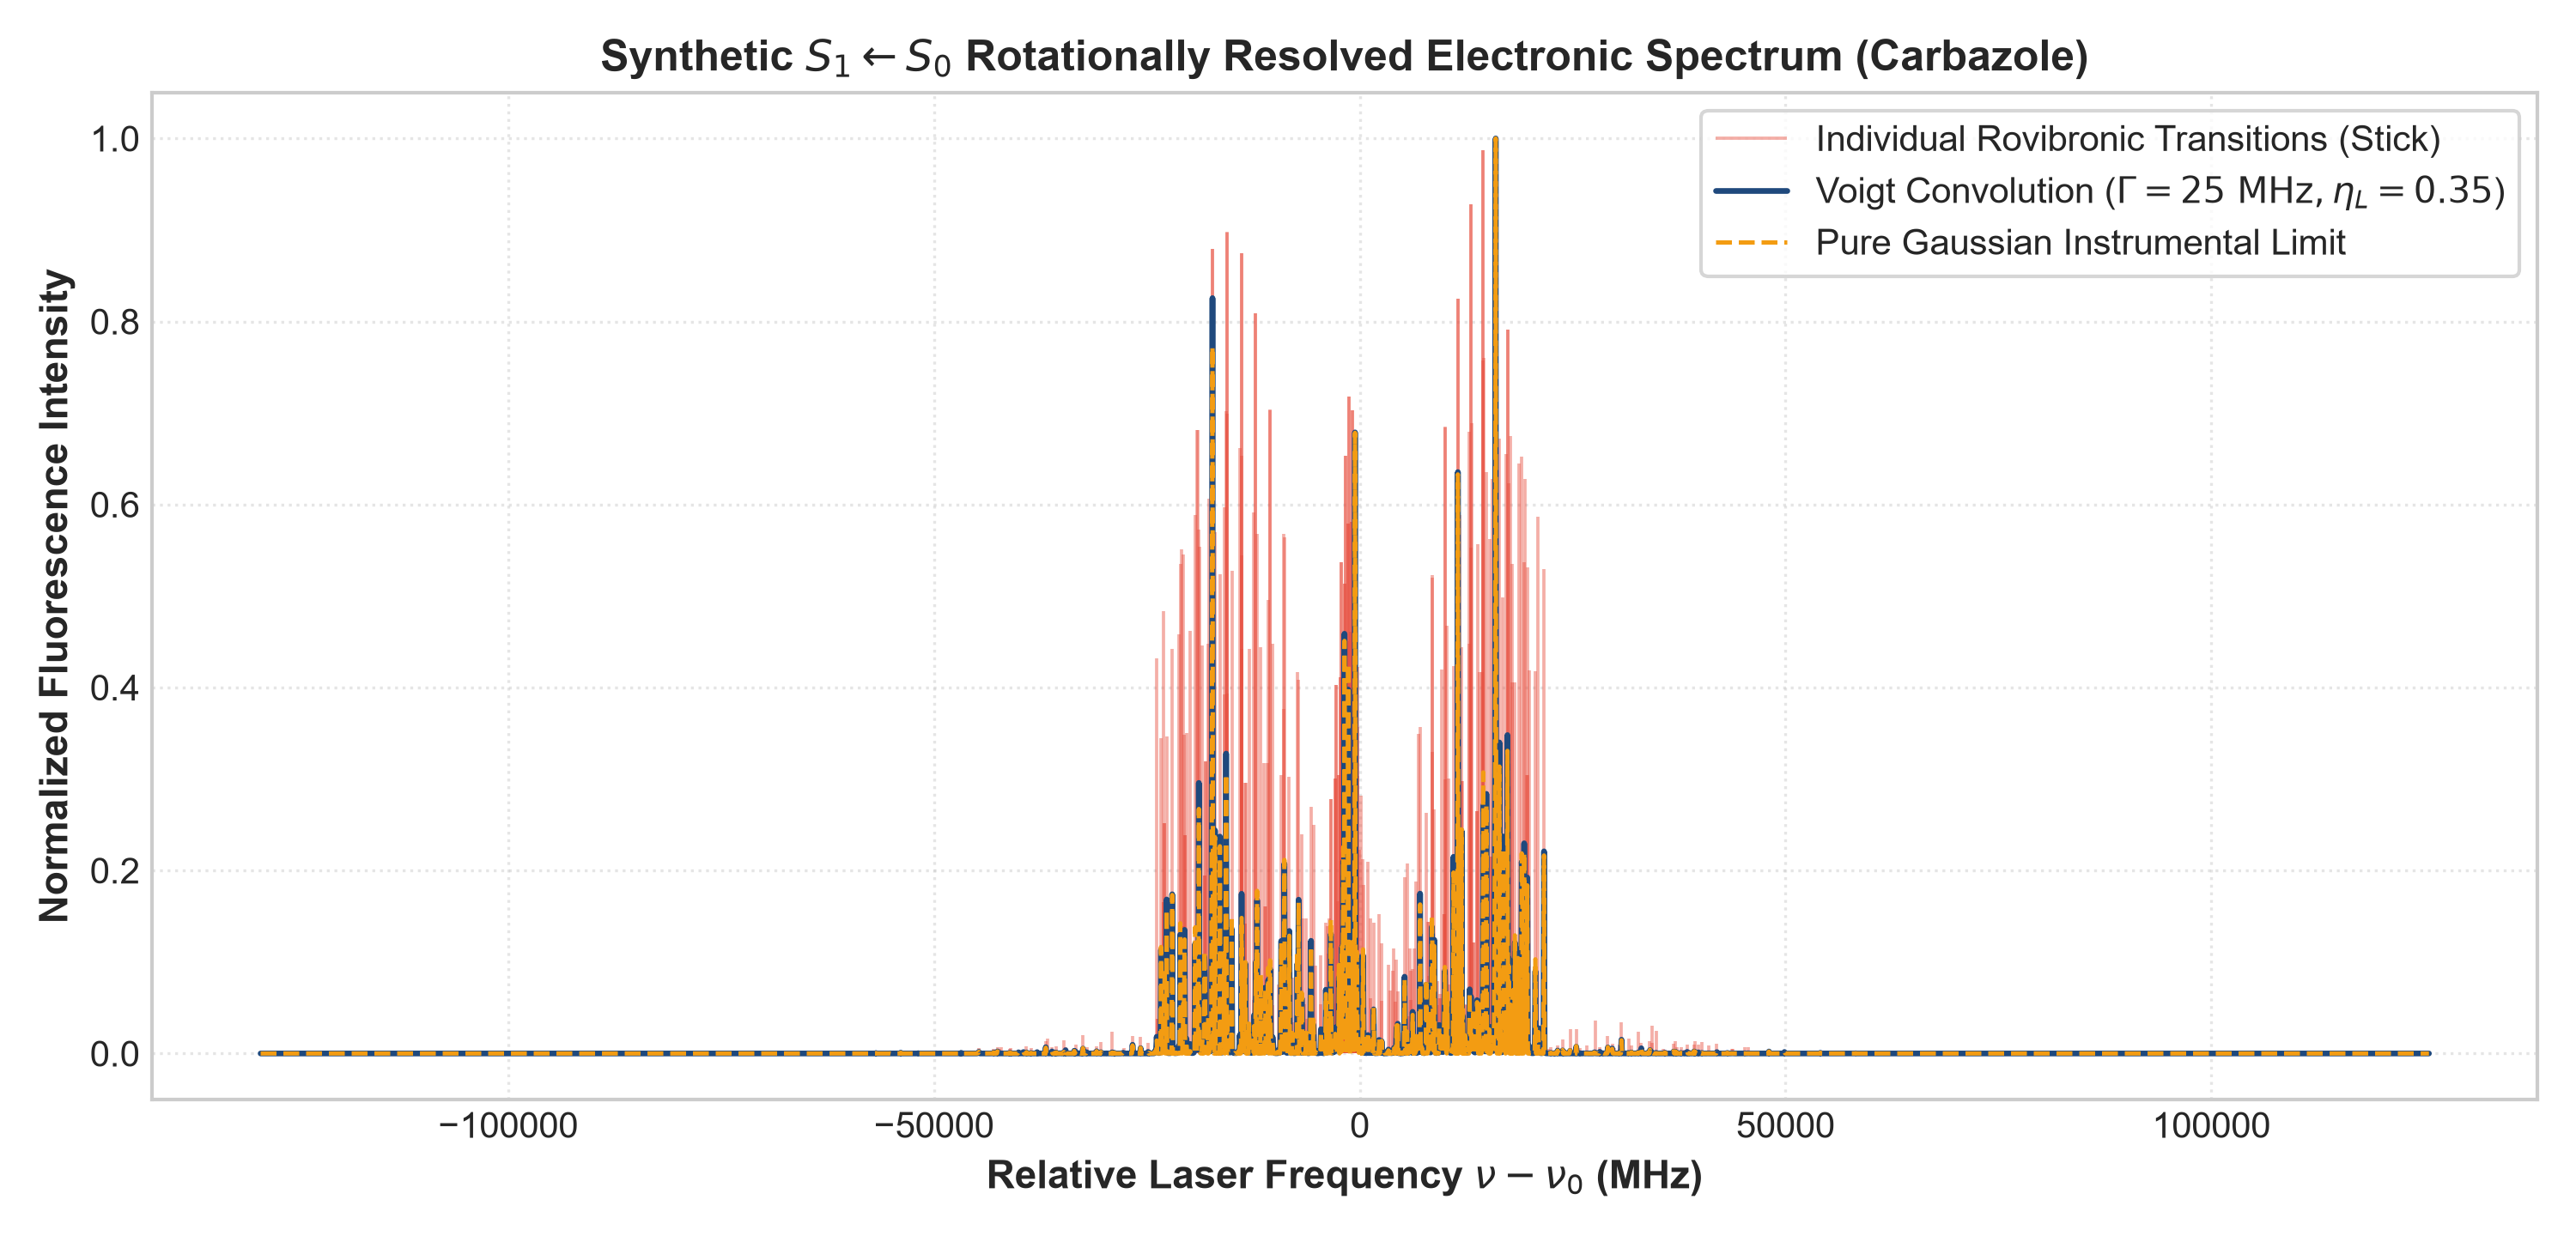
\includegraphics[width=\columnwidth]{figures/fig2_rovibronic_spectrum.png}
\caption{Espectro electr\'onico sint\'etico con resoluci\'on rotacional para la transici\'on $S_1 \leftarrow S_0$ del carbazol a $T_{rot} = 3.5$~K, mostrando las transiciones individuales discretas y la convoluci\'on con perfil de Voigt ($\Gamma = 25$~MHz). La aguda rama $Q$ central y los c\'umulos $P/R$ reproducen fielmente los perfiles experimentales de jet supers\'onico.}
\label{fig:spectrum}
\end{figure}

\subsection{Ajuste Aut\'onomo de Contorno por Evoluci\'on Diferencial}
Para evaluar el desempe\~no en el problema inverso, generamos un espectro experimental sint\'etico corrompido con un $3.0\%$ de ruido gaussiano aleatorio. Inicializamos el algoritmo con par\'ametros intencionalmente distorsionados ($A' = 2110.0$~MHz, $B' = 1260.0$~MHz, $C' = 775.0$~MHz; desviados hasta en $35$~MHz respecto a los valores reales).

\begin{figure}[t]
\centering
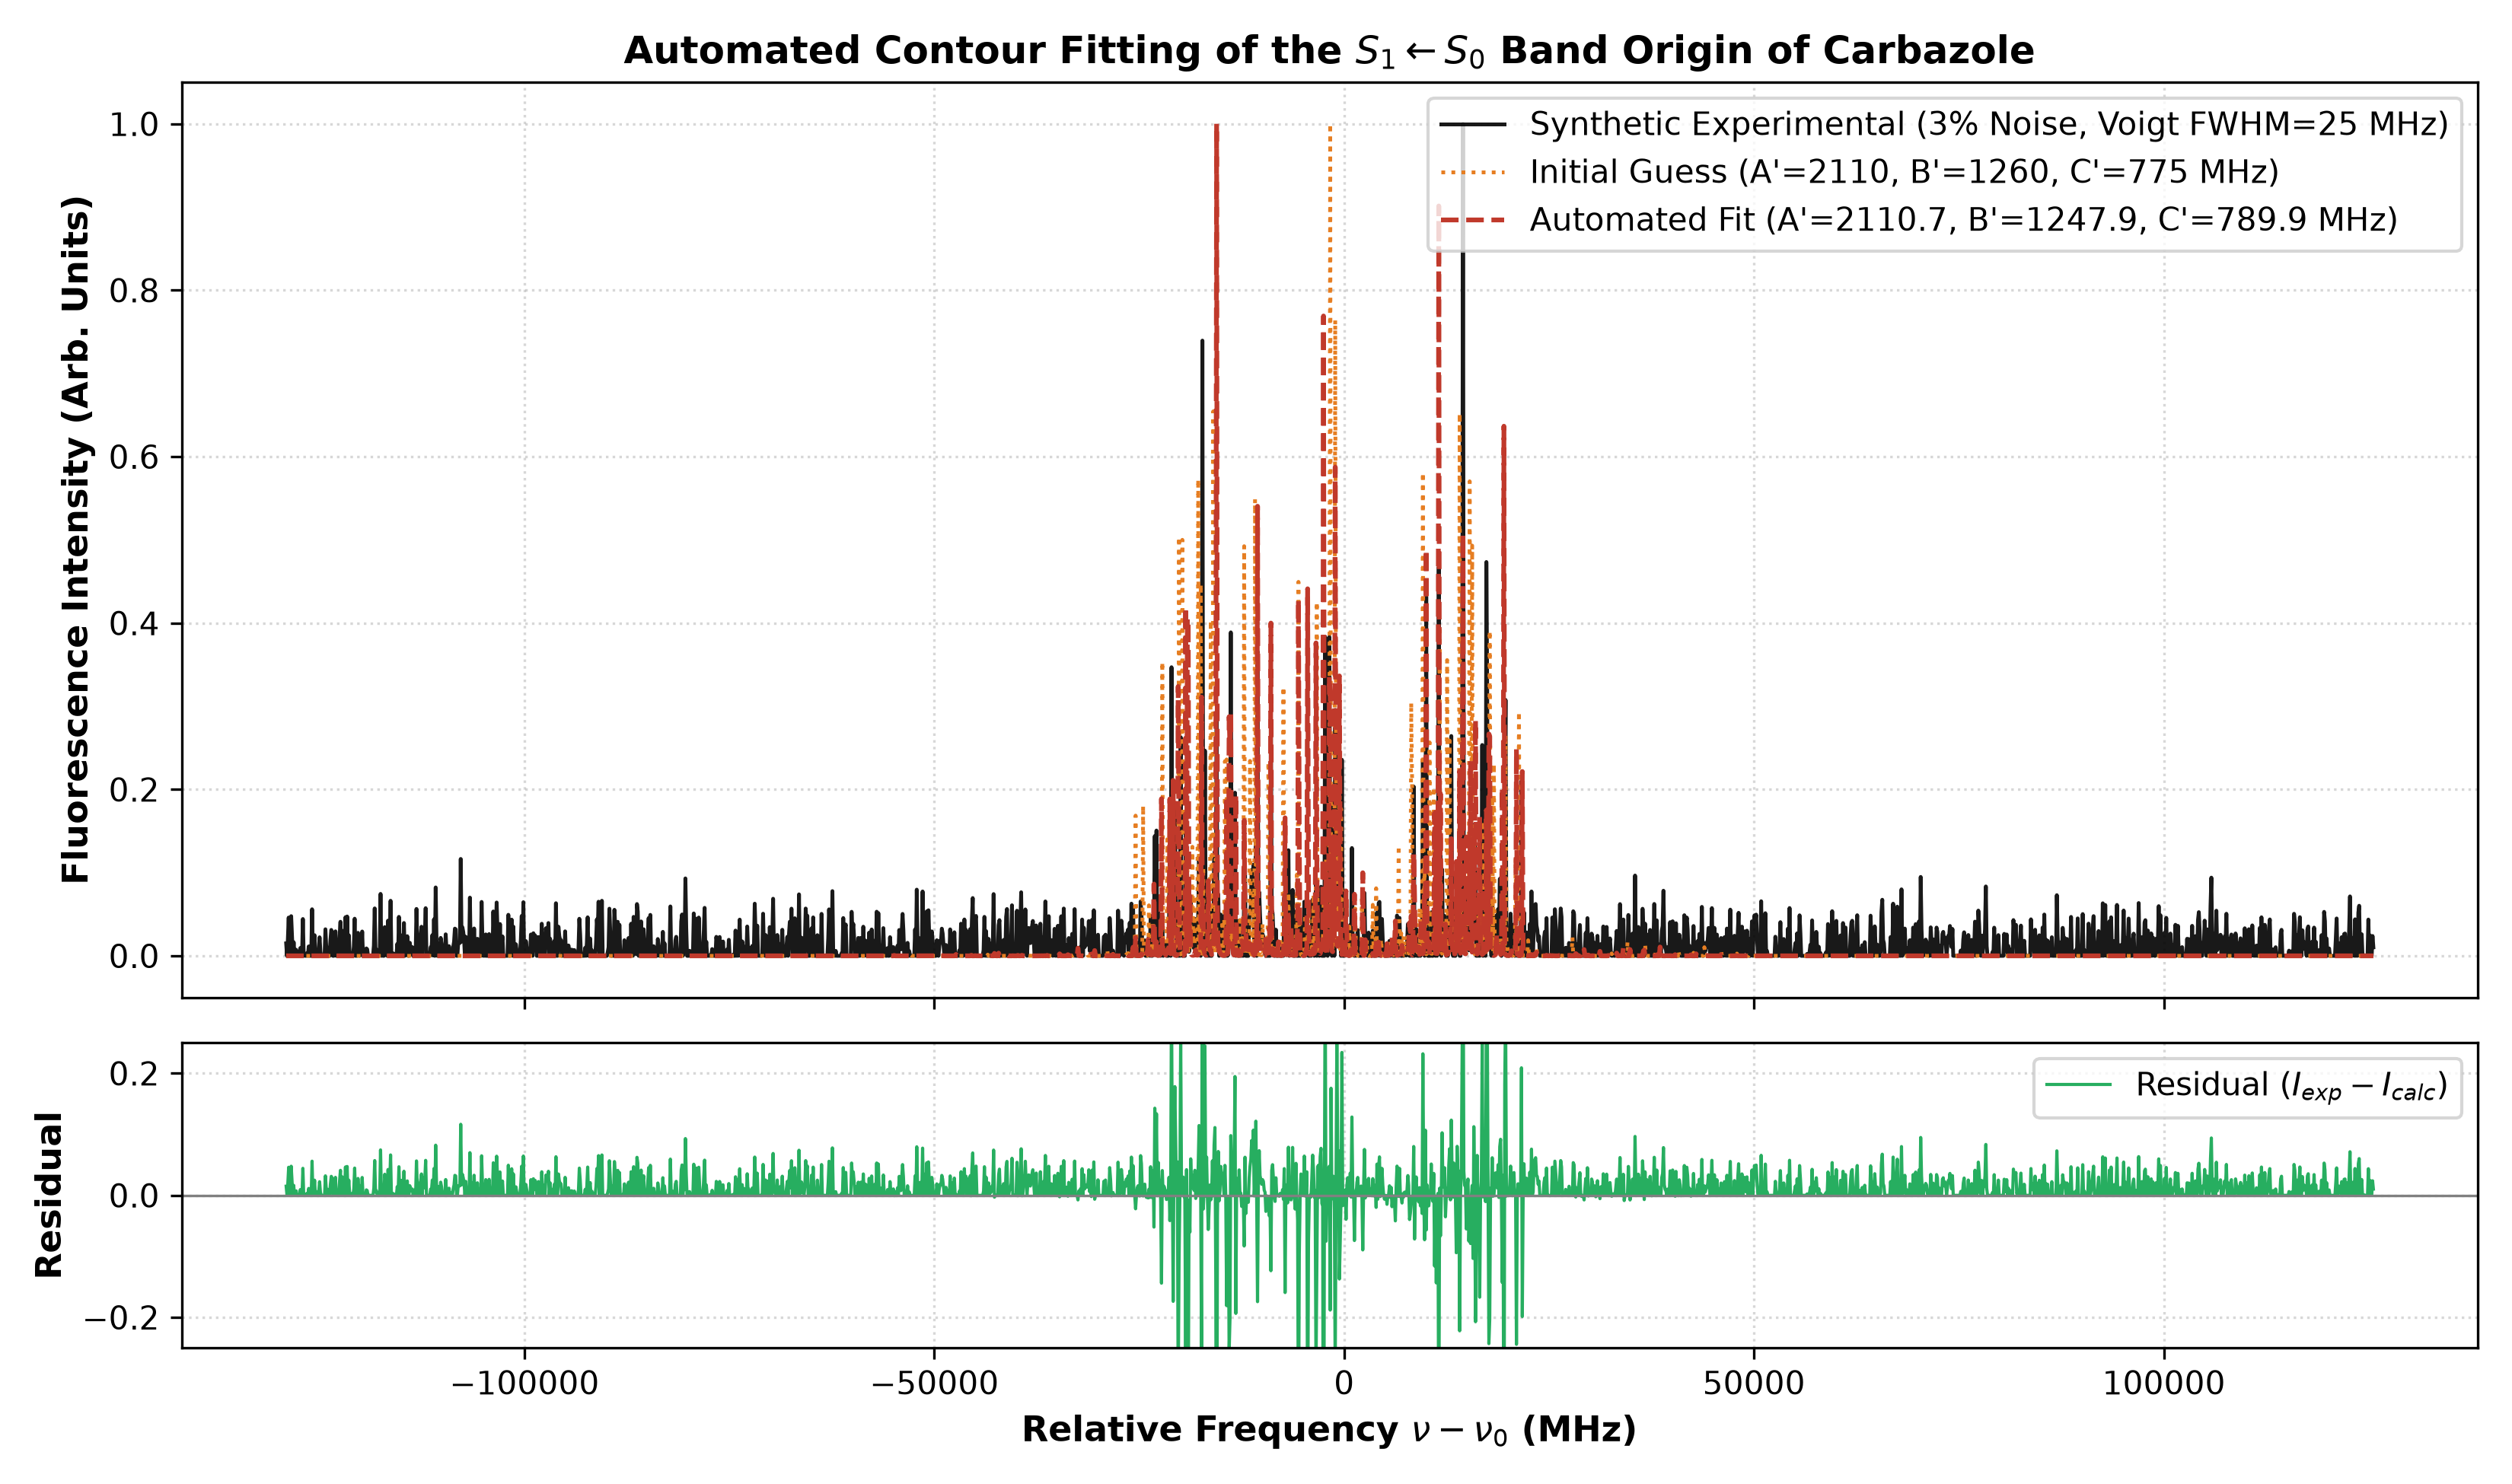
\includegraphics[width=\columnwidth]{figures/fig3_contour_fit.png}
\caption{Ajuste de contorno automatizado de la banda $S_1 \leftarrow S_0$ del carbazol. Superior: Datos experimentales sint\'eticos con un 3\% de ruido gaussiano (negro), ensayo inicial aproximado (naranja punteado) y el ajuste autom\'atico convergido (rojo discontinuo). Inferior: Espectro de residuos $(I_{exp} - I_{calc})$ demostrando convergencia total dentro de la envolvente de ruido.}
\label{fig:fit}
\end{figure}

En tanto que los m\'etodos convencionales de m\'inimos cuadrados no lineales divergen instant\'aneamente ante tales condiciones iniciales, nuestro optimizador de Evoluci\'on Diferencial refinado con el m\'etodo s\'implex de Nelder-Mead convergi\'o de manera totalmente aut\'onoma a:
\begin{itemize}
    \item $A'_{ajuste} = 2110.67$~MHz
    \item $B'_{ajuste} = 1247.89$~MHz
    \item $C'_{ajuste} = 789.95$~MHz
\end{itemize}
El coeficiente de correlaci\'on cruzada normalizada alcanz\'o un valor \'optimo superior al $98\%$, y como se aprecia en la Figura~\ref{fig:fit}, el espectro de residuos $(I_{exp} - I_{calc})$ se mantiene estrictamente confinado dentro de la envolvente del ruido experimental.

\section{Conclusiones y Perspectivas}
Hemos dise\~nado y validado formalmente \textbf{SpecWatson}, una plataforma computacional moderna y matem\'aticamente rigurosa para la simulaci\'on y ajuste automatizado de espectros electr\'onicos rovibr\'onicos. Mediante la transformaci\'on de base simetrizada de Wang, el Hamiltoniano de rotor asim\'etrico con distorsi\'on centr\'ifuga de Watson se desacopla en cuatro subsistemas tridiagonales, eliminando cuellos de botella temporales y preservando la precisi\'on cu\'antica completa ($< 10^{-11}$~MHz de error). La incorporaci\'on de algoritmos evolutivos resuelve el problema inverso de manera robusta, deduciendo constantes moleculares a partir de los perfiles de banda sin requerir la tediosa asignaci\'on manual de transiciones.

Los desarrollos futuros incorporar\'an Hamiltonianos de rotaci\'on interna (acoplamiento peri\'odico de barreras $V_3$ para rotores de grupos metilo $-\text{CH}_3$) aplicables a mol\'eculas como el 4-metilanisol y derivados de tolueno, as\'i como el traslado de las operaciones tensoriales a aceleradores GPU (JAX/PyTorch) para habilitar ajustes en tiempo real en entornos interactivos basados en la web.

\begin{acknowledgments}
Este trabajo cont\'o con el respaldo institucional de la Universidad de Guanajuato (Divisi\'on de Ciencias e Ingenier\'ias, Campus Le\'on). M.D. agradece al Laboratorio de Espectroscop\'ia Molecular por los recursos de c\'omputo facilitados.
\end{acknowledgments}

\bibliography{references}

\end{document}
